\documentclass{article}
\usepackage{tikz}
\usetikzlibrary{matrix}

\begin{document}

\begin{center}
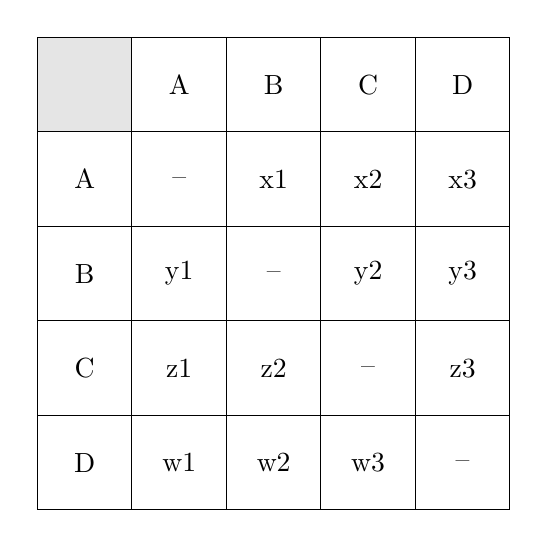
\begin{tikzpicture}
\matrix[matrix of nodes,
        nodes={draw, minimum size=1.2cm, anchor=center},
        column sep=-\pgflinewidth, row sep=-\pgflinewidth] (m) {
    |[fill=gray!20]|   & A & B & C & D \\
    A & -- & x1 & x2 & x3 \\
    B & y1 & -- & y2 & y3 \\
    C & z1 & z2 & -- & z3 \\
    D & w1 & w2 & w3 & -- \\
};
\end{tikzpicture}
\end{center}

\end{document}